\documentclass[journal]{IEEEtran}

\usepackage{graphicx}


\usepackage{cite}
\usepackage{amsmath}
\usepackage{multirow}
\usepackage{algpseudocode}


\hyphenation{}


\begin{document}

\title{Action Execution Alters Action Perception:\\ A Computational Approach}

\author{\IEEEauthorblockN{Jimmy Baraglia, Jorge L. Copete, Yukie Nagai, and Minoru Asada}\\
\IEEEauthorblockA{Graduate School of Engineering, Osaka University\\
2-1 Yamada-oka, Suita, Osaka, 565-0871 Japan \\
Email:  \{jimmy.baraglia,jorge.copete,yukie,asada\}@ams.eng.osaka-u.ac.jp}

\thanks{No thanks}}

% The paper headers
\markboth{Journal of \LaTeX\ Class Files,~Vol.~13, No.~9, September~2014}%
{Shell \MakeLowercase{\textit{et al.}}: Bare Demo of IEEEtran.cls for Journals}

\maketitle

% As a general rule, do not put math, special symbols or citations
% in the abstract or keywords.
\begin{abstract}
The perception of others' motions as goal directed actions has been shown to emerge in infants as they become able to manipulate their environments. Hence, it has been shown though infant studies that the perception of action can be altered 3-months-old toddler by allowing them to interact with object using sticky mittens.  

\end{abstract}

% Note that keywords are not normally used for peerreview papers.
\begin{IEEEkeywords}
Cognitive robotics, action perception, recurrent neural network
\end{IEEEkeywords}


\section{Introduction}

\begin{itemize}
\item Sommerville et al., 2005 \cite{Sommerville2005} Action experience alters 3-month-old infants' perception of others' actions.
\item Gerson et al., 2014 \cite{gerson2014learning} Results revealed a unique effect of active over observational experience. Furthermore, findings suggest that benefits of trained actions do not generalize broadly, at least following brief training.
\item Hunnius and Bekkering \cite{hunnius2014you} Action experience is an important process through which infants develop the capacity of action understanding
\end{itemize}

\section{Hypothesis 1: Perception via Action} 
\begin{itemize}
\item Meltzoff \cite{meltzoff2007like} Infants represent the acts of others and their own acts in commensurate terms. They can recognize cross-modal equivalences between acts they see others perform and their own felt bodily movements. 
\item Minoto et al., 2010 \cite{Minato2012} The simulated infants are able to develop the components of a healthy body mapping in order, that is, relating self motion first, followed by an understanding of others’ motions, which is supported by psychological studies.
\item rizzolatti and sinigaglia \cite{rizzolatti2010functional} Recent findings show that the parieto-frontal mirror circuit in monkeys encodes the goal of the observed motor acts. In humans, there is evidence that the same circuit encodes the goal of the observed motor act and its individual movements.
\item Uithol et al. \cite{uithol2011mirror} It is unlikely that a direct mirroring process is by itself capable of processing context in all its complexity
\end{itemize}

\section{Hypothesis 2: Attention Model}
\begin{itemize}
\item Kidd et al., 2012 \cite{Kidd2012} Human infants allocate attention to visual sequences that are neither too simple nor too complex.
\item Nagai et al., 2015 \cite{nagai2015model} Infants have a fixed preference function: higher for a moderate prediction error, and lower for a smaller/larger prediction error.
\end{itemize}

\section{Conclusion}

\bibliographystyle{ieeetr}
\bibliography{TAMD_babybot}

\begin{IEEEbiography}[{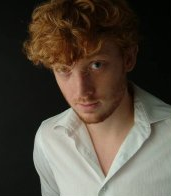
\includegraphics[width=1in,height=1.25in,clip,keepaspectratio]{figures/picture}}]{Jimmy Baraglia}
received his Bachelor degree in Electronics and Industrial Computer Science. In September 2012, he got his masters' degree in Intelligent System Engineering from Toulouse 3 University, during which he researched on the emergence of the mirror neurons systems. In October 2012, he started a PhD course in Cognitive Robotics at the Osaka University in which he attended to several exchange courses in Germany and in Italy. His research interest is to understand the emergence of pro-social behavior in young infants and to create robots able to develop similar abilities.
\end{IEEEbiography}

\begin{IEEEbiography}[{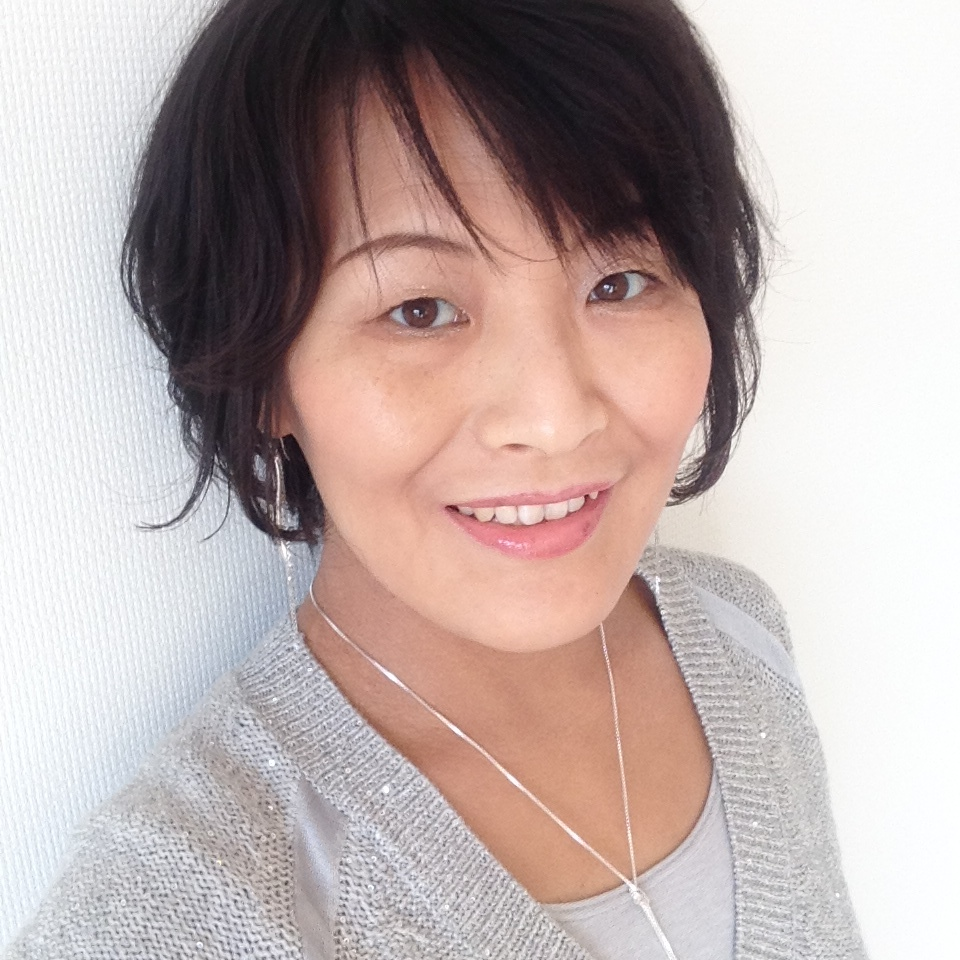
\includegraphics[width=1in,height=1.25in,clip,keepaspectratio]{figures/pictureNagai}}]{Yukie Nagai}
is a Specially Appointed Associate Professor at Osaka University, Japan. She received her Ph.D. in Engineering from Osaka University in 2004 and worked as a postdoc researcher at National Institute of Information and Communications Technology in Kyoto from 2004 to 2006. She then worked at Bielefeld University, Germany for three and a half years until she started her current position at Osaka University in October 2009. Her research interests include the developmental mechanism of human social cognition such as self-other cognition, imitation, joint attention, and cooperation. She has been investigating the underlying mechanisms for cognitive development by means of constructive approaches.
\end{IEEEbiography}

\begin{IEEEbiography}[{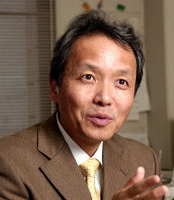
\includegraphics[width=1in,height=1.25in,clip,keepaspectratio]{figures/pictureAsada}}]{Minoru Asada}
became Professor at Osaka University in April 1995. Since April 1997, he has been Professor in the Department of Adaptive Machine Systems at the Graduate School of Engineering, Osaka University. Dr. Asada has received many awards such as the Best Paper award at the IEEE/RSJ International Conference on Intelligent Robots and Systems (IROS92) and the Commendation by the Minister of Education, Culture, Sports, Science and Technology, Japanese Government as Person of Distinguished Services to Enlightening People on Science and Technology. He is one of the founders of RoboCup, and the former president of the International RoboCup Federation (2002-2008). Since 2005, he has been Research Director of “ASADA Synergistic Intelligence Project” at Exploratory Research for Advanced Technology by Japan Science and Technology Agency (ERATO), and is currently, a principal investigator of Grants-in-Aid for Scientific Research (Research Project Number: 24000012 (2012-2016)) titled “Constructive Developmental Science based on Understanding the Process from Neurodynamics to Social Interaction.”
\end{IEEEbiography}

\end{document}


